\documentclass[12pt]{beamer}

\usepackage[brazil]{babel}
\usepackage[utf8]{inputenc}
\usepackage[T1]{fontenc}
\usepackage{animate}
\usepackage{amsbsy}
\usepackage{amsfonts}
\usepackage{amsmath}
\usepackage{amssymb}
\usepackage{amsthm}
\setbeamertemplate{theorems}[numbered] % to number
\usepackage[toc,page,title,titletoc]{appendix}
\usepackage{dsfont}
\usepackage{esvect}
\usepackage[labelfont=bf]{caption}
%\usepackage{subcaption}
\usepackage{float}
\usepackage[Glenn]{fncychap}%Sonny %Conny %Lenny %Glenn %Renje %Bjarne %Bjornstrup
\usepackage{graphicx}
\usepackage{subfig}
\usepackage{indentfirst}%Para indentar os paragrafos automáticamente
\usepackage{lipsum}
\usepackage{longtable}
\usepackage{mathtools}
\usepackage{listings}%Inserir codigo do R no latex
\usepackage{multirow}
\usepackage{multicol}
\usepackage{csquotes}
\usepackage[maxcitenames=2,terseinits=true,natbib=true, style=authoryear, maxbibnames=99]{biblatex}
\addbibresource{../Referencias/Referencias.bib}
\usepackage[figuresright]{rotating}
\usepackage{spalign}
\usepackage{pgfplots}
\pgfplotsset{compat=1.17}
\usepackage{tikz}
\usepackage{fontawesome}
\usepackage{color, colortbl}
\usepackage{url}
\usepackage{cancel}
\usepackage{accents}
\usepackage{bm}
\usepackage{ragged2e}%para justificar o texto dentro de algum ambiente
\definecolor{Gray}{gray}{0.9}
\definecolor{LightCyan}{rgb}{0.88,1,1}


\usepackage[all]{xy}
\usepackage{hyperref,bookmark}
\hypersetup{
  colorlinks=true,
  linkcolor=blue,
  citecolor=red,
  filecolor=blue,
  urlcolor=blue,
}

\usetheme{Madrid}
\usecolortheme[RGB={193,0,0}]{structure}

%\setbeamertemplate{footline}[frame number]
%\setbeamertemplate{footline}[text line]{%
%  \parbox{\linewidth}{\vspace*{-8pt}\hfill\date{}\hfill\insertshortauthor\hfill\insertpagenumber}}
\beamertemplatenavigationsymbolsempty
\renewcommand{\vec}[1]{\mbox{\boldmath$#1$}}
\newtheorem{Teorema}{Teorema}
\newtheorem{Proposicao}{Proposição}
\newtheorem{definicao}{Definição}
\newtheorem{Corolario}{Corolário}
\newtheorem{Demonstracao}{Demonstração}
\newcommand{\bx}{\ensuremath{\bar{x}}}
\newcommand{\Ho}{\ensuremath{H_{0}}}
\newcommand{\Hi}{\ensuremath{H_{1}}}
\newcommand{\at}[2][]{#1|_{#2}}
\newcommand\xuparrow[1][2ex]{%
   \mathrel{\rotatebox{-90}{$\xleftarrow{\rule{#1}{0pt}}$}}
}
\apptocmd{\frame}{}{\justifying}{} % Allow optional arguments after frame.

\makeatletter
\setbeamertemplate{footline}
{
  \leavevmode%
  \hbox{%
  \begin{beamercolorbox}[wd=.3\paperwidth,ht=2.25ex,dp=1ex,center]{author in head/foot}%
    \usebeamerfont{author in head/foot}\mytext
  \end{beamercolorbox}%
  \begin{beamercolorbox}[wd=.3\paperwidth,ht=2.25ex,dp=1ex,center]{title in head/foot}%
    \usebeamerfont{title in head/foot}\mytextt
  \end{beamercolorbox}%
  \begin{beamercolorbox}[wd=.35\paperwidth,ht=2.25ex,dp=1ex,right]{site in head/foot}%
    \usebeamerfont{site in head/foot}\mytexttt\hspace*{2em}
    \insertframenumber{} / \inserttotalframenumber\hspace*{2ex} 
  \end{beamercolorbox}}%
  \vskip0pt%
}
\makeatother

\providecommand{\arcsin}{} \renewcommand{\arcsin}{\hspace{2pt}\textrm{arcsen}}
\providecommand{\sin}{} \renewcommand{\sin}{\hspace{2pt}\textrm{sen}}
\newcommand{\N}{\rm I\!N}
\newcommand{\I}{\rm I\!I}
\newcommand{\R}{\rm I\!R}
\newcommand{\Sim}{\overset{\text{iid}}{\sim}}
\newcommand{\Lim}{{\displaystyle \lim_{n\to\infty}}}
\newcommand{\LimInf}{{\displaystyle \liminf_{n\to\infty}}}
\newcommand{\rightLim}{\xrightarrow[n\rightarrow\infty]{}}
\newcommand{\Sumi}{{\displaystyle \sum_{i=1}^{n}}}
\newcommand{\Int}{{\displaystyle \int_{-\infty}^{+\infty}}}
\newcommand{\ConvD}{\overset{D}{\rightarrow}}
\newcommand{\ConvP}{\overset{P}{\rightarrow}}
\newcommand{\Prodi}{{\displaystyle \prod_{i=1}^{n}}}
\newcommand{\SetaUP}[2]{\underset{\mathclap{\substack{\xuparrow[30pt] \\ #1}}}{#2}}
%\newcommand{\SetaInclinada}[2]{\underset{\mathclap{\substack{\rotatebox{135}{\xuparrow[30pt] \\ #1}}}}{#2}}
\newcommand{\Home}{\begin{tikzpicture}
\node[scale=2] at (3,4) {\text{Para}~\faHome};
\end{tikzpicture}}
\newcommand{\vecX}{\boldsymbol{X}}
\newcommand{\Implica}[1]{\xRightarrow{#1}}
\newcommand{\SeSe}{\iff}
\newcommand{\EscoreA}{\dfrac{\partial}{\partial\theta}\log{f(x,\theta)}}
\newcommand{\EscoreB}{\dfrac{\partial^{2}}{\partial\theta^{2}}\log{f(x,\theta)}}
\newcommand{\cqd}{\text{cqd}~\blacksquare}
\newcommand{\seqX}{$X_{1},\ldots,X_{n}$}
\newcommand{\seqY}{$Y_{1},\ldots,Y_{n}$}
\newcommand{\tend}[1]{\hbox{\oalign{$\bm{#1}$\crcr\hidewidth$\scriptscriptstyle\bm{\sim}$\hidewidth}}}

%\newtheorem{Teorema}{Teorema}
%\newtheorem{Proposicao}{Proposição}
%\newtheorem{Definicao}{Definição}
%\newtheorem{Corolario}{Corolário}
%\newtheorem{Demonstracao}{Demonstração}

\titlegraphic{\hspace*{8cm}\href{https://fsbmat-ufv.github.io/}{
\includegraphics[width=2cm]{figs/mylogo.png}}
}

%Continuar a numeracao em slides diferentes
\newcounter{saveenumi}
\newcommand{\seti}{\setcounter{saveenumi}{\value{enumi}}}
\newcommand{\conti}{\setcounter{enumi}{\value{saveenumi}}}

\resetcounteronoverlays{saveenumi}

% Layout da pagina
\hypersetup{pdfpagelayout=SinglePage}

%Para o \pause funcionar dentro do ambiente align
\makeatletter
\let\save@measuring@true\measuring@true
\def\measuring@true{%
  \save@measuring@true
  \def\beamer@sortzero##1{\beamer@ifnextcharospec{\beamer@sortzeroread{##1}}{}}%
  \def\beamer@sortzeroread##1<##2>{}%
  \def\beamer@finalnospec{}%
}
\makeatother

\title{Inferência Estatística II}
\author{Prof. Fernando de Souza Bastos\texorpdfstring{\\ fernando.bastos@ufv.br}{}}
\institute{Departamento de Estatística\texorpdfstring{\\ Programa de Pós-Graduação em Estatística Aplicada e Biometria}\texorpdfstring{\\ Universidade Federal de Viçosa}{}\texorpdfstring{\\ Campus UFV - Viçosa}{}}
\date{}
\newcommand\mytext{Aula 13}
\newcommand\mytextt{Fernando de Souza Bastos}
\newcommand\mytexttt{\url{https://est711.github.io/}}


\begin{document}
%\SweaveOpts{concordance=TRUE}

\frame{\titlepage}

\begin{frame}{}
\frametitle{\bf Sumário}
\tableofcontents
\end{frame}


\section{Introdução}
\begin{frame}{Teste Qui-Quadrado}
\begin{block}{}
\justifying

Testes qui-quadrado foram originalmente proposto por Karl Pearson em 1900, este teste representou um dos primeiros métodos de inferência estatística. Considere a variável aleatória $X_i$ distribuída como $N(\mu_i, \sigma^2_i)$, em que $i = 1, 2, \ldots, n$, e as variáveis $X_1, X_2, \ldots, X_n$ mutuamente independentes. A função de densidade conjunta dessas variáveis é dada por:

\[
f(x_1, x_2, \ldots, x_n) = \frac{1}{\sigma_1 \ldots \sigma_n (2\pi)^{n/2}} e^{\left( -\dfrac{1}{2} {\displaystyle \sum_{i=1}^{n}} \left(\frac{x_i - \mu_i}{\sigma_i}\right)^2 \right)}, -\infty < x_i < \infty
\]
\end{block}
\end{frame}

\begin{frame}{}
\begin{block}{}
\justifying
A variável aleatória definida pelo expoente (exceto o coeficiente -1/2) é a soma ${\displaystyle \sum_{i=1}^{n}} \left(\frac{x_i - \mu_i}{\sigma_i}\right)^2$, essa variável aleatória segue uma distribuição Qui-Quadrado com $n$ graus de liberdade, denotada como $\chi^2(n)$. 
\end{block}
\end{frame}

\section{Resultado Importante}
\begin{frame}{Prove que $Z^2\sim \chi^{2}(1)$}
\begin{block}{}
\justifying
Considere $V=Z^{2}.$ Quero mostrar que a densidade de $V$ é a densidade de uma variável qui-quadrado com 1 grau de liberdade, dada por:
\begin{align*}
    g(v)=\dfrac{1}{2^{\frac{1}{2}}\Gamma\left(\dfrac{1}{2}\right)}v^{\frac{1}{2}-1}e^{-\frac{v}{2}},~v>0
\end{align*}
\end{block}
\pause
\begin{block}{}
\justifying
Para mostrar tal resultado, notem que 
\begin{align*}
    G(v)&=P(V\leq v)=P(Z^{2}\leq v)\\
    &=P(-\sqrt{v}\leq Z\leq \sqrt{v})\\
    &=2P(0\leq Z\leq \sqrt{v}),~Z~\text{é simétrica em relação a origem!}\\
    &=2{\displaystyle\int_{0}^{\sqrt{v}}}\dfrac{1}{\sqrt{2\pi}}e^{-\frac{z^{2}}{2}}dz
\end{align*}
\end{block}
\end{frame}

\begin{frame}{}
\begin{block}{}
\justifying
Considere $z=\sqrt{y}\Rightarrow~dz=\dfrac{y^{-\frac{1}{2}}}{2}dy=\dfrac{1}{2\sqrt{y}}dy,$ nesse caso, $z=0\Rightarrow~y=0,~z^{2}\Rightarrow~y=v,$ logo, 
\end{block}
\pause
\begin{block}{}
\justifying
\begin{align*}
    G(v)&=2{\displaystyle\int_{0}^{\sqrt{v}}}\dfrac{1}{\sqrt{2\pi}}e^{-\frac{z^{2}}{2}}dz\\
    &=2{\displaystyle\int_{0}^{v}}\dfrac{1}{\sqrt{2\pi}}e^{-\frac{y}{2}}\dfrac{1}{2\sqrt{y}}dy\\
    &=2{\displaystyle\int_{0}^{v}}\dfrac{1}{\sqrt{\pi}\sqrt{2}}y^{\frac{1}{2}-1}e^{-\frac{y}{2}}dy,~v>0
\end{align*}
\end{block}
\pause 
\begin{block}{}
\justifying
Segue que,
\begin{align*}
    G^{'}(v)&=g(v)=\dfrac{1}{\sqrt{\pi}\sqrt{2}}v^{\frac{1}{2}-1}e^{-\frac{v}{2}}dy,~v>0
\end{align*}
\end{block}
\end{frame}

\begin{frame}{}
\begin{block}{}
\justifying
Usando o fato de $\Gamma\left(\dfrac{1}{2}\right)=\sqrt{\pi},$ temos que,
\begin{align*}
   g(v)=\dfrac{1}{\Gamma\left(\dfrac{1}{2}\right)\sqrt{2}}v^{\frac{1}{2}-1}e^{-\frac{v}{2}}dy,~v>0~\cqd
\end{align*}

\end{block}
\end{frame}

\section{Teorema}
\begin{frame}{}
\begin{Teorema}
\justifying
Sejam $Z_1, Z_2, \ldots, Z_{\nu}$ variáveis aleatórias independentes com distribuição normal padrão, onde $\nu$ é um inteiro positivo. Então, a variável aleatória $\chi^2(\nu) = {\displaystyle \sum_{i=1}^{\nu}} Z_i^2$ segue uma distribuição qui-quadrado com $\nu$ graus de liberdade.
\end{Teorema}
\pause
\begin{block}{Observação:}
\justifying
A soma de duas variáveis qui-quadrado independentes, $\chi^2(\nu_1) + \chi^2(\nu_2)$, segue uma distribuição qui-quadrado com $\nu_1 + \nu_2$ graus de liberdade.
\end{block}
\end{frame}

\begin{frame}{}
\begin{block}{}
\justifying
Devido aos resultados anteriores, se $X_1$ segue uma distribuição binomial $b(n, p_1)$, considere a variável aleatória:

\[
Y = \frac{X_1 - np_1}{\sqrt{np_1(1 - p_1)}}
\]
\end{block}
\pause
\begin{block}{}
\justifying
Conforme $n$ se aproxima do infinito, a variável $Y$ tem uma distribuição aproximada $N(0, 1).$ Além disso, a distribuição de $Y^2$ é aproximadamente $\chi^2(1)$.
\end{block}
\end{frame}

\begin{frame}{}
\begin{block}{}
\justifying
Seja $X_2 = n - X_1$ e $p_2 = 1 - p_1$. Defina $Q_1=Y^{2},$ então

\[
Q_1 = \frac{(X_1 - np_1)^2}{np_1(1 - p_1)} = \frac{(X_1 - np_1)^2}{np_1} + \frac{(X_2 - np_2)^2}{np_2}
\]

Isso ocorre porque $(X_1 - np_1)^2 = (n - X_2 - n + np_2)^2 = (X_2 - np_2)^2$. 
\end{block}
\end{frame}

\begin{frame}{}
\begin{block}{}
\justifying
Esse resultado pode ser generalizado da seguinte maneira. Suponha que $X_1, X_2, \ldots, X_{k-1}$ tenham uma distribuição multinomial com os parâmetros $n$ e $p_1, p_2, \ldots, p_{k-1}$. Defina $X_k = n - (X_1 + X_2 + \ldots + X_{k-1})$ e $p_k = 1 - (p_1 + p_2 + \ldots + p_{k-1})$. Defina $Q_{k-1}$ por:

\[
Q_{k-1} = \sum_{i=1}^{k} \frac{(X_i - n p_i)^2}{n p_i}
\]

À medida que $n$ se aproxima do infinito, $Q_{k-1}$ possui uma distribuição aproximada $\chi^2(k - 1)$. Para usar essa aproximação, é importante garantir que $n$ seja grande o suficiente para que cada $n p_i$, onde $i = 1, 2, \ldots, k$, seja pelo menos igual a 5.
\end{block}
\end{frame}

\section{Teste Qui-Quadrado}
\begin{frame}{Teste Qui-Quadrado}
\begin{block}{}
\justifying
Considere um espaço amostral $A$ de um experimento aleatório que seja a união de $k$ conjuntos mutuamente disjuntos $A_1, A_2, \ldots, A_k$. Suponha que $P(A_i) = p_i,~i = 1, 2, \ldots, k$, e $p_k = 1 - p_1 - p_2 - \ldots - p_{k-1}$. Em que $p_i$ é a probabilidade de que o resultado do experimento aleatório seja um elemento do conjunto $A_i$.
\end{block}
\pause
\begin{block}{}
\justifying
Repita um experimento aleatório $n$ vezes de forma independente, e considere $X_i$ como o número de vezes que o resultado do experimento é um elemento do conjunto $A_i$. Ou seja, $X_1, X_2, \ldots, X_k = n - X_1 - X_2 - \ldots - X_{k-1}$ representam as frequências com as quais o resultado é, respectivamente, um elemento de $A_1, A_2, \ldots, A_k$. A função de massa de probabilidade conjunta de $X_1, X_2, \ldots, X_{k-1}$ é a função de massa de probabilidade multinomial com os parâmetros $n, p_1, p_2, \ldots, p_{k-1}$.    
\end{block}
\end{frame}


\begin{frame}{}
\begin{block}{}
\justifying
Considere a hipótese simples:
\begin{align*}
    H_0: p_1 &= p_{10}, p_2 = p_{20}, \ldots, p_{k-1} = p_{k-1,0}\\ 
    (p_k &= p_{k0} = 1 - p_{10} - p_{20} - \ldots - p_{k-1,0})
\end{align*}

Em que $p_{10}, p_{20}, \ldots, p_{k-1,0}$ são valores especificados. Deseja-se testar $H_0$ em relação a todas as alternativas.  
\end{block}
\pause
\begin{block}{}
\justifying
Se a hipótese $H_0$ for verdadeira, a variável aleatória

\[
Q_{k-1} = \sum_{i=1}^{k} \frac{(X_i - n p_{i0})^2}{n p_{i0}}
\]
tem uma distribuição aproximada qui-quadrado com $k - 1$ graus de liberdade. Pois, se $H_0$ é verdadeira, $n p_{i0}$ é o valor esperado de $X_i.$ Os valores observados de $Q_{k-1}$ não devem ser muito grandes se $H_0$ for verdadeira.
\end{block}
\end{frame}

\begin{frame}{}
\begin{block}{}
\justifying
Podemos, portanto, considerar o teste com nível de significância $\alpha$ que rejeita $H_0$ quando $Q_{k-1} \geq c.$ Usando o software R, calculamos o valor crítico $c$ por meio da função \texttt{qchisq(1 - $\alpha$, k - 1)}. Se a hipótese $H_0$ for rejeitada quando o valor observado de $Q_{k-1}$ for pelo menos igual a $c$, o teste de $H_0$ terá um nível de significância aproximadamente igual a $\alpha$. Além disso, se $q$ for o valor realizado da estatística do teste $Q_{k-1}$, o nível de significância observado do teste pode ser calculado em R pela função \texttt{1-pchisq(q, k - 1)}. Isso é frequentemente chamado de teste de bondade de ajuste. 

\end{block}
\end{frame}

\section{Exemplo 1}
\begin{frame}{Exemplo 1}
\begin{block}{}
\justifying
Escolher um dos seis primeiros números inteiros positivos por meio de um experimento aleatório (por exemplo, lançamento de um dado). Seja $A_i = \{x : x = i\}$, onde $i = 1, 2, \ldots, 6$. 

$$H_0 : P(A_i) = p_{i0} = \frac{1}{6},~i = 1, 2, \ldots, 6,$$ 

$\alpha=5\%$. Para realizar o teste, o experimento aleatório é repetido sob as mesmas condições, 60 vezes de forma independente. Ou seja, $k = 6$ e $n \cdot p_{i0} = 60 \cdot \frac{1}{6} = 10,~i = 1, 2, \ldots, 6$. Seja $X_i$ a frequência com que o experimento aleatório termina com o resultado em $A_i,~i = 1, 2, \ldots, 6$. Defina $Q_5$ como:

\[
Q_5 = \sum_{i=1}^{6} \frac{(X_i - 10)^2}{10}
\]

\end{block}
\end{frame}

\begin{frame}{}
\begin{block}{}
\justifying
Uma vez que existem $6 - 1 = 5$ graus de liberdade, o valor crítico para um teste com nível $\alpha = 0.05$ é $qchisq(0.95, 5) = 11.0705$. Suponha agora que as frequências experimentais de $A_1, A_2, \ldots, A_6$ sejam, respectivamente, 13, 19, 11, 8, 5 e 4. O valor observado de $Q_5$ é calculado como:

\begin{align*}
Q_{5,cal} &= \frac{(13 - 10)^2}{10} + \frac{(19 - 10)^2}{10} + \frac{(11 - 10)^2}{10}\\ 
&+ \frac{(8 - 10)^2}{10} + \frac{(5 - 10)^2}{10} + \frac{(4 - 10)^2}{10}\\ 
&= 15.6
\end{align*}

Como $15.6 > 11.0705$, a hipótese $P(A_i) = \frac{1}{6},~i = 1, 2, \ldots, 6$, é rejeitada a um nível de significância (aproximado) de $5\%.$
\end{block}
\end{frame}

\begin{frame}{}
\begin{block}{}
\begin{figure}
    \centering
    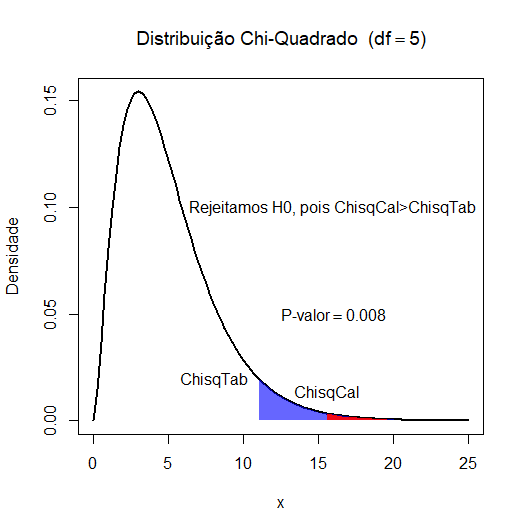
\includegraphics[scale=0.5]{figs/EX1Chisq.png}
    \caption{Gráfico com Resultados do Teste Qui-Quadrado}
    \label{fig:enter-label}
\end{figure}
\end{block}
\end{frame}

\begin{frame}{}
\begin{block}{}
\begin{figure}
    \centering
    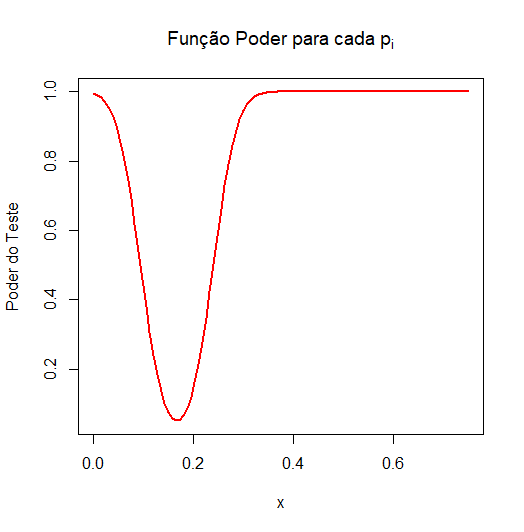
\includegraphics[scale=0.5]{figs/EX1Poder.png}
    \caption{Poder do Teste Qui-Quadrado (Exemplo 1)}
    \label{fig:enter-label}
\end{figure}
\end{block}
\end{frame}

\section{Exemplo 2}
\begin{frame}{Exemplo 2}
\begin{block}{}
\justifying
Neste exemplo, um ponto deve ser selecionado a partir do intervalo unitário $\{x : 0 < x < 1\}$ por meio de um processo aleatório. Definimos os conjuntos $A_1 = \{x : 0 < x \leq \dfrac{1}{4}\}$, $A_2 = \{x : \dfrac{1}{4} < x \leq \dfrac{1}{2}\}$, $A_3 = \{x : \dfrac{1}{2} < x \leq \dfrac{3}{4}\}$ e $A_4 = \{x : \dfrac{3}{4} < x < 1\}$. As probabilidades $p_i$, onde $i = 1, 2, 3, 4$, atribuídas a esses conjuntos sob a hipótese são determinadas pela função de densidade de probabilidade $2x$, em que $0 < x < 1$, e zero caso contrário. Essas probabilidades são:
\begin{align*}
    p_{10} &= \int_{0}^{\frac{1}{4}} 2x \, dx = \frac{1}{16},\quad p_{20} = \int_{\frac{1}{4}}^{\frac{1}{2}} 2x \, dx = \frac{3}{16}\\
    p_{30} &= \int_{\frac{1}{2}}^{\frac{3}{4}} 2x \, dx = \frac{5}{16}\quad~
    p_{40} = \int_{\frac{3}{4}}^{1} 2x \, dx = \frac{7}{16}
\end{align*}

\end{block}
\end{frame}

\begin{frame}{}
\begin{block}{}
\justifying
Portanto, a hipótese a ser testada é que $p_1, p_2, p_3$ e $p_4 = 1 - p_1 - p_2 - p_3$ possuem os valores anteriores em uma distribuição multinomial com $k = 4$. Considere $\alpha=0.025$, repetindo o experimento aleatório $n = 80$ vezes de forma independente sob as mesmas condições, temos $n \cdot p_{i0},~i = 1, 2, 3, 4$ são, respectivamente, $5, 15, 25$ e $35.$
\end{block}
\pause
\begin{block}{}
\justifying
Suponha que as frequências observadas de $A_1, A_2, A_3$ e $A_4$ sejam 6, 18, 20 e 36, respectivamente. Assim, 
\begin{align*}
    Q_{3,cal}&=\frac{(6 - 5)^2}{5} + \frac{(18 - 15)^2}{15} + \frac{(20 - 25)^2}{25} + \frac{(36 - 35)^2}{35} = \frac{64}{35}\\ 
    &\approx 1.83.
\end{align*}
Ou seja, falhamos em rejeitar $H_{0},$ pois $\chi_{tab}^{2}=qchisq(0.975,3)=9.34.$
\end{block}
\end{frame}

\begin{frame}{}
\begin{block}{}
\begin{figure}
    \centering
    \includegraphics[scale=0.5]{figs/EX2Chisq.png}
    \caption{Gráfico com Resultados do Teste Qui-Quadrado}
    \label{fig:enter-label}
\end{figure}
\end{block}
\end{frame}

\begin{frame}{}
\begin{block}{}
\begin{figure}
    \centering
    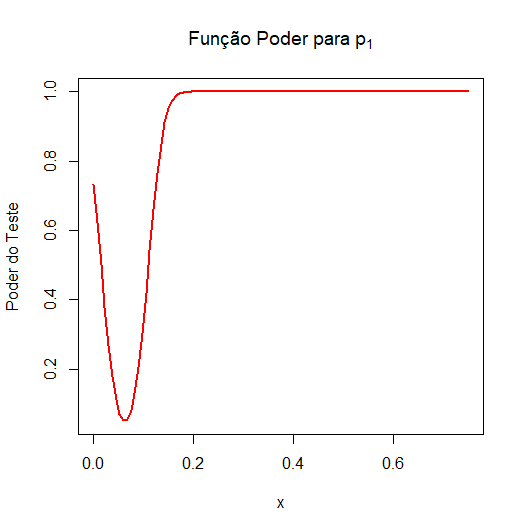
\includegraphics[scale=0.5]{figs/Ex2p1.png}
    \caption{Poder do Teste Qui-Quadrado (Exemplo 2)}
    \label{fig:enter-label}
\end{figure}
\end{block}
\end{frame}

\begin{frame}{}
\begin{block}{}
\begin{figure}
    \centering
    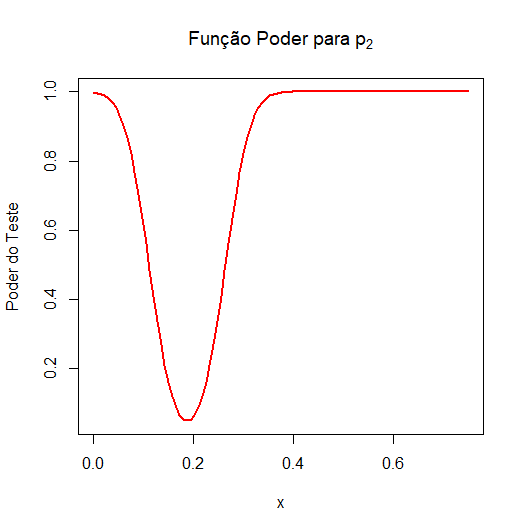
\includegraphics[scale=0.5]{figs/Ex2p2.png}
    \caption{Poder do Teste Qui-Quadrado (Exemplo 2)}
    \label{fig:enter-label}
\end{figure}
\end{block}
\end{frame}

\begin{frame}{}
\begin{block}{}
\begin{figure}
    \centering
    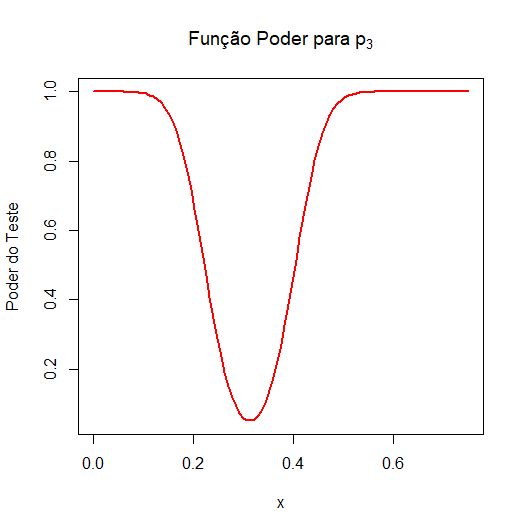
\includegraphics[scale=0.5]{figs/Ex2p3.png}
    \caption{Poder do Teste Qui-Quadrado (Exemplo 2)}
    \label{fig:enter-label}
\end{figure}
\end{block}
\end{frame}

\begin{frame}{}
\begin{block}{}
\begin{figure}
    \centering
    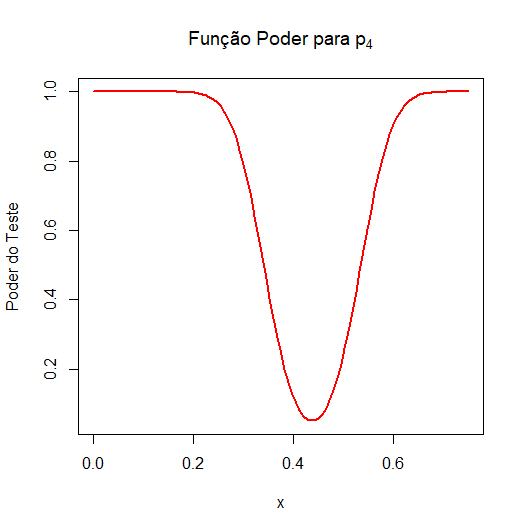
\includegraphics[scale=0.5]{figs/Ex2p4.png}
    \caption{Poder do Teste Qui-Quadrado (Exemplo 2)}
    \label{fig:enter-label}
\end{figure}
\end{block}
\end{frame}


\begin{frame}{\Home}
\begin{block}{}
\justifying

\begin{itemize}
    \item \textbf{Exercícios da seção 4.7:} 1, 4 e 9.
\end{itemize}
\nocite{hogg}
\end{block}
\end{frame}

\section{Distribuição F}
\begin{frame}{Distribuição F}
\begin{definicao}
\justifying
Sejam $Y$ e $W$ variáveis aleatórias independentes, em que $Y$ segue uma distribuição qui-quadrado com $m$ graus de liberdade e $W$ segue uma distribuição qui-quadrado com $n$ graus de liberdade, $m$ e $n$ inteiros positivos dados. Defina uma nova variável aleatória $X$ da seguinte forma:

\[
X = \dfrac{Y/m}{W/n} = \frac{nY}{mW}.
\]

Então, a distribuição de $X$ é chamada de distribuição $F$ com $m$ e $n$ graus de liberdade. A função de densidade de probabilidade da distribuição F é apresentada no próximo slide.
\end{definicao}
\end{frame}

\begin{frame}{}
\begin{block}{}
\justifying
Seja $X$ uma variável aleatória com distribuição $F$ com $m$ e $n$ graus de liberdade. Então, sua função de densidade de probabilidade $f(x)$ é a seguinte, para $x > 0:$

\[
f(x) = \dfrac{\Gamma\left[\frac{1}{2}(m+n)\right]m^{m/2}n^{n/2}}{\Gamma\left[\frac{1}{2}m\right]\Gamma\left[\frac{1}{2}n\right]}\dfrac{x^{m/2}-1}{(mx+n)^{(m+n)/2}},
\]
e $f(x) = 0$ para $x \geq 0.$

\end{block}
\end{frame}

\section{Teste F}
\begin{frame}{}
\begin{block}{}
\justifying
Suponha que as variáveis aleatórias $X_1, \ldots, X_m$ formem uma amostra aleatória de $m$ observações de uma distribuição normal para a qual tanto a média $\mu_1$ quanto a variância $\sigma^2_1$ são desconhecidas. Suponha também que as variáveis aleatórias $Y_1, \ldots, Y_n$ formem uma amostra aleatória independente de $n$ observações de outra distribuição normal para a qual tanto a média $\mu_2$ quanto a variância $\sigma^2_2$ são desconhecidas. Por fim, suponha que as seguintes hipóteses devam ser testadas a um nível de significância especificado $\alpha_0$ ($0 < \alpha_0 < 1$):

\[
H_0: \sigma^2_1 \leq \sigma^2_2, \quad H_1: \sigma^2_1 > \sigma^2_2.
\]
\end{block}
\end{frame}

\begin{frame}{}
\begin{block}{}
\justifying
Definimos $S^2_X$ e $S^2_Y$ como as variâncias amostrais de $X$ e $Y,$ respectivamente. Então, $S^2_X / (m - 1)$ e $S^2_Y / (n - 1)$ são estimadores de $\sigma^2_1$ e $\sigma^2_2$, respectivamente. Faz sentido intuitivo rejeitar $H_0$ se a razão desses dois estimadores for grande. Ou seja, definimos

\[
V = \frac{S^2_X}{m - 1} \bigg/ \frac{S^2_Y}{n - 1},
\]

e rejeitamos $H_0$ se $V \geq c$, onde $c$ é escolhido para que o teste tenha um nível de significância desejado.

\end{block}
\end{frame}

\subsection{Exemplo 1}
\begin{frame}{Exemplo 1}
\begin{block}{}
\justifying
Suponha que seis observações $X_1, \ldots, X_6$ sejam selecionadas aleatoriamente de uma distribuição normal para a qual tanto a média $\mu_1$ quanto a variância $\sigma^2_1$ são desconhecidas, e é encontrado que $S^2_X = 30$. Suponha também que 21 observações, $Y_1, \ldots, Y_{21}$, sejam selecionadas aleatoriamente de outra distribuição normal para a qual tanto a média $\mu_2$ quanto a variância $\sigma^2_2$ são desconhecidas, e é encontrado que $S^2_Y = 40$. Realize um teste F das hipóteses 
\[
H_0: \sigma^2_1 \leq \sigma^2_2, \quad H_1: \sigma^2_1 > \sigma^2_2.
\].

\end{block}
\end{frame}

\begin{frame}{}
\begin{block}{}
\justifying
Neste exemplo, temos $m = 6$ e $n = 21$. Portanto, quando $H_0$ é verdadeira, a estatística $V$, seguirá a distribuição $F$ com $5$ e $20$ graus de liberdade. Segue que o valor de $V$ para as amostras dadas é
$V = \frac{30/5}{40/20} = 3$.

O valor-p do teste, pode ser calculado no R por:

\begin{align*}
    Pvalor&=P(F>Tcal)\\
    &=pf(Fcal,nx-1,ny-1,lower.tail=FALSE)=0.035
\end{align*}

A hipótese $H_0$ de que $\sigma^2_1 \leq \sigma^2_2$ seria, portanto, rejeitada no nível de significância $\alpha_0 = 0.05$, e $H_0$ não seria rejeitada no nível de significância $\alpha_0 = 0.025$. 
\end{block}
\end{frame}

\begin{frame}{}
\begin{block}{}
\justifying
É possível mostrar que o poder deste teste pode ser escrito como:

\begin{align*}
    \gamma_{d}(\sigma_{1}^{2},\sigma_{2}^{2})=1-F_{m-1,n-1}(C*\dfrac{\sigma_{1}^{2}}{\sigma_{2}^{2}}), C=F_{tab}
\end{align*}

Suponha, assim, que seja importante rejeitar $H_0$ se $\sigma^2_1$ for três vezes maior que $\sigma^2_2$. Nesse caso, gostaríamos que a função poder fosse alta quando $\sigma^2_1 = 3\sigma^2_2$. Nesse caso, $1 - F_{5,20}(2.71 \times 1/3) \approx 0.5$. Logo, se $\sigma^2_1$ for três vezes maior que $\sigma^2_2$, o teste com nível de 0.05 tem cerca de 50\% de chance de rejeitar $H_0$.
\end{block}
\end{frame}

\begin{frame}[allowframebreaks]
\frametitle{\bf Referências}
\printbibliography
\end{frame}


\end{document}
